\documentclass[12pt,twoside,openright]{report}

%\usepackage{mathptmx}
\usepackage[utf8]{inputenc}
\usepackage[english]{babel}
\usepackage[pdftex]{graphicx}
\usepackage[a4paper,width=150mm,top=25mm,bottom=25mm,bindingoffset=6mm]{geometry}
\usepackage{fancyhdr}
\usepackage[backend=bibtex,sorting=none,citestyle=numeric-comp]{biblatex}
\usepackage{mathtools}
\usepackage{amsmath}
\usepackage[font={small}]{caption}
\usepackage{bm}
\usepackage{titlesec}
\usepackage{emptypage}
\usepackage{times}


% PRE CONFIGURATIONS

\titleformat{\chapter}
  {\normalfont\LARGE\bfseries}{\thechapter.}{1em}{}
\graphicspath{{images/}}
\addbibresource{references.bib}
\setlength{\headheight}{14.5pt}
\pagestyle{fancy}
\fancyhead[RO,LE]{}
\fancyhead[LO]{\thechapter.\space\leftmark}
\fancyhead[RE]{\rightmark}
\renewcommand{\chaptermark}[1]{\markboth{\uppercase{#1}}{}}
\bibliography{references}
\DefineBibliographyStrings{english}{%
  bibliography = {References},
}

\renewcommand{\figurename}{\small Figure}
\newcommand{\figureref}[1]{Fig. \ref{fig:#1}}
\newcommand{\equationref}[1]{Eq. \ref{eq:#1}}
\newcommand{\chapterref}[1]{Chapter \ref{ch:#1}}
\newcommand{\sectionref}[1]{Section \ref{sec:#1}}

%MATH COMMANDS
\newcommand{\dvec}[1]{\boldsymbol{#1}}
\newcommand{\dhatvec}[1]{\boldsymbol{\hat{#1}}}
\newcommand{\prob}[1]{P(#1)}
\newcommand{\postprob}[2]{P(#1|#2)}
\newcommand{\pdf}[1]{p(#1)}
\newcommand{\postpdf}[2]{p(#1|#2)}
\newcommand{\verifytest}[2]
{
    \left\{
        \begin{array}{ll}
            \geq #1, & \text{accept } #2,\\
            < #1, & \text{reject } #2.
        \end{array}
    \right.
}
\newcommand{\verifytestB}[2]
{
    \left\{
        \begin{array}{ll}
            \geq #1, & \text{accept } #2,\\
            < #1, & \text{reject } #2,
        \end{array}
    \right.
}


%GLOBAL DEFINITIONS

\gdef\universityname{Universidade Federal de Pernambuco}
\gdef\centername{Centro de Informática}
\gdef\papertitle{A Fractional Gaussian Mixture Model for Speaker Verification}
\gdef\papertype{Final Term Paper}
\gdef\authorname{Eduardo Martins Barros de Albuquerque Tenório}
\gdef\advisername{Tsang Ing Ren}
\gdef\adviserfullname{Prof. Dr. \advisername}
\gdef\defensedate{March 3, 2015}


\title{
    {
\includegraphics{ufpelogo.png}}
    \\
    {\large \universityname}
    \\
    {\large \centername}
    \vfill
    \textbf{\papertitle}
    \vskip\baselineskip
    {\large \papertype}
    \vfill
}
\author{\authorname}
\date{\normalsize\vfill \defensedate}


\begin{document}
\pagenumbering{gobble}
\maketitle


%FRONTMATTER

\chapter*{Declaration}
This paper is a presentation of my original research work, as partial fulfillment of the requirement for the degree in Computer Engineering. Wherever contributions of others are involved, every effort is made to indicate this clearly, with due reference to the literature, and acknowledgement of collaborative research and discussions.
\vskip\baselineskip
\noindent The work was done under the guidance of \adviserfullname, at Centro de Informática, Universidade Federal de Pernambuco, Brazil.

\vskip5\baselineskip
\begin{flushright}
\rule{0.75\textwidth}{1pt}
\vskip0.5\baselineskip
Eduardo Martins Barros de Albuquerque Tenório
\end{flushright}

\vskip2\baselineskip
\noindent In my capacity as supervisor of the candidate’s paper, I certify that the above statements are true to the best of my knowledge.

\vskip5\baselineskip
\begin{flushright}
\rule{0.75\textwidth}{1pt}
\vskip0.5\baselineskip
\adviserfullname
\end{flushright}

\vfill
\begin{center}
\defensedate
\end{center}

\chapter*{Acknowledgements}
I am thankful to my parents, for the support and patience during the graduation,\\
To my adviser, Tsang Ing Ren, for the guidance,\\
To Cleice Souza and Leonardo Brito, for the previous readings and help.

\chapter*{}
\vfill
\begin{flushright}
    \textit{Live long and prosper}\\
    \vskip0.5\baselineskip
    Vulcan salute
\end{flushright}
\vfill

\chapter*{Abstract}
TODO escrever o abstract após terminar tudo (após a conclusão).\\

\tableofcontents
\pagenumbering{roman}


%MIDDLEMATTER

\section{Introdução}
\label{sec:intro}

\contentscurrent

\begin{frame}
\frametitle{Reconhecimento de ...}
\begin{description}
    \item[Fala] \textbf{O que} está sendo dito
    \pause
    \begin{itemize}
        \item Conteúdo da mensagem
        \pause
        \item Estado emocional do locutor
        \pause
        \item Sotaque ou dificuldade de articulação
        \pause
    \end{itemize}
    \item[Locutor] \textbf{Quem} está falando
    \pause
    \begin{itemize}
        \item Identificar uma pessoa na multidão
        \pause
        \item Autenticar um usuário
        \pause
    \end{itemize}
    \item Este trabalho é focado em \textbf{reconhecimento de locutor}
\end{description}
\end{frame}

\subsection{Reconhecimento de Locutor}

\begin{frame}
\frametitle{Reconhecimento de Locutor}
\begin{description}
    \item[Identificação] Determina a identidade de um locutor dentro de um conjunto não unitário
    \pause
    \begin{itemize}
        \item 1 para N
        \pause
        \item Problema de \textbf{conjunto fechado}
        \pause
    \end{itemize}
    \item[Verificação] Determina se o locutor é quem diz ser
    \pause
    \begin{itemize}
        \item 1 para 1
        \pause
        \item Problema de \textbf{conjunto aberto}
        \pause
    \end{itemize}
\end{description}

\begin{figure}
    \centering
    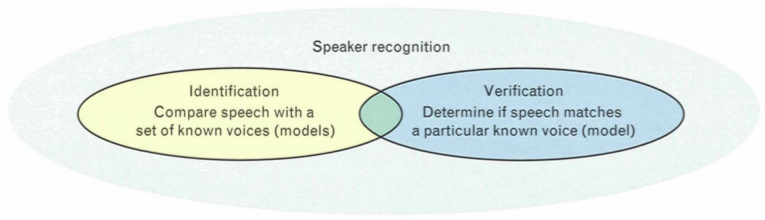
\includegraphics[width=0.75\textwidth]{speaker-recognition}
\end{figure}
\end{frame}

\begin{frame}
\frametitle{Dependência de texto}
\begin{description}
    \item[Dependente] Teste $\in$ Treinamento
    \pause
    \begin{itemize}
        \item Diversos graus de dependência
        \pause
        \item Teste $\not\in$ Treinamento $\implies$ Retreinamento
        \pause
    \end{itemize}
    \item[Independente] Teste $\neq$ Treinamento
    \pause
    \begin{itemize}
        \item Características não textuais
        \pause
        \item Presentes em diferentes sotaques e até \emph{gibberish}
    \end{itemize}
    \pause
    \item Este trabalho é focado em \textbf{reconhecimento de locutor independente de texto}
\end{description}
\end{frame}

\subsection{Modelos de Mistura Gaussiana}

\begin{frame}
\frametitle{Modelos de Mistura Gaussiana}
\begin{description}
    \item[GMM] Combinação de Gaussianas
    \pause
    \item[UBM] GMM gerado por diversas locuções de fundo
    \pause
    \item[AGMM] GMM adaptado a partir de um UBM
    \pause
    \item[FGMM] GMM utilizando Fractional Covariance Matrix (FCM)
\end{description}
\end{frame}

\subsection{Objetivos}

\begin{frame}
\frametitle{Objetivos}
\begin{description}
    \item Implementar sistemas de reconhecimento de locutor e analizar
    \pause
    \begin{itemize}
        \item Taxas de \textbf{sucesso} para identificação
        \pause
        \begin{itemize}
            \item Diferentes tamanhos de mistura ($M$)
            \pause
            \item Diferentes tamanhos de características
            \pause
        \end{itemize}
        \item Comparar identificação utilizando GMM e FGMM
        \pause
        \item Taxas de \textbf{falsa detecção} e \textbf{falsa rejeição} para verificação
        \pause
        \begin{itemize}
            \item Diferentes tamanhos de mistura ($M$)
            \pause
            \item Diferentes tamanhos de características
            \pause
        \end{itemize}
        \item Comparar verificação utilizando GMM e AGMM
    \end{itemize}
\end{description}
\end{frame}

\chapter{Speaker Recognition Systems}

The process of voice recognition lies on the field of pattern classification, with the speaker and his or her utterance (a speech signal) as inputs for a classifier and a decision as output. This decision may be, given an utterance $\boldsymbol{Y}$ produced by a speaker $\mathcal{S}$ and a set $\boldsymbol{\mathcal{S}} = \{\mathcal{S}_1, ..., \mathcal{S}_S\}$ of known users,

\begin{equation}
    \mathcal{S} \gets \mathcal{S}_i \text{, if } i = \arg\max_j P(\mathcal{S}_j|\boldsymbol{Y}).
    \label{eq:decision_speaker_identification}
\end{equation}

\noindent This is a case of speaker identification and the output is a $\mathcal{S}_i$ from $\boldsymbol{\mathcal{S}}$. Another type of decision is

\begin{equation}
    \text{if } P(\mathcal{S}_i|\boldsymbol{Y}) \verifytest{\alpha}{\mathcal{S}}
    \label{eq:decision_speaker_verification}
\end{equation}

\noindent This is a speaker verification decision, with a binary output, given a $\mathcal{S}$ who produced $\boldsymbol{Y}$, a claimed identity $\mathcal{S}_i$ from $\boldsymbol{\mathcal{S}}$ and a threshold $\alpha$ for acceptance. This chapter (and indirectly the whole document) is about the type of decision from \equationref{decision_speaker_verification}.

\section{Basic Concepts}

\subsection{Utterance}

An utterance is a piece of speech produced by a speaker. It may be a word, a statement or any vocal sound. The terms \emph{utterance} and \emph{speech signal} sometimes are used interchangeably, but here speech signal will be associated to an utterance recorded and digitalized. An example of an utterance as speech signal is shown in \figureref{speech_signal}.

\begin{figure}[ht]
    \centering
    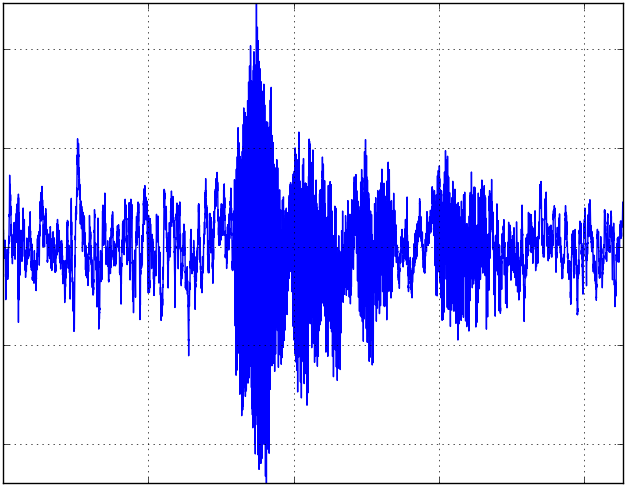
\includegraphics[width=\textwidth]{speech_signal}
    \caption{Speech signal for utterance ``karen livescu".}
    \label{fig:speech_signal}
\end{figure}

\subsection{Features}

The raw speech signal is unfit for usage by a recognition system. For a correct processing, the unique features from the speaker's vocal tract are extracted, reducing the number of variables the system needs to deal with (leading to a simpler implementation) and performing a better evaluation (just use the necessary informations). This extraction is executed by the MFCC algorithm, explained in \chapterref{feature-extraction}. Due to the stationary properties of the speech signal when analyzed in a short period of time, it is divided in overlapping frames of small and predefined length, to avoid ``loss of significancy" in the features \cite{davis.mermelstein.1980, rabiner.schafer.2007}.

\subsection{Dependency x Independency}

\section{Likelihood Ratio Test}

TODO basear-se na seção 2 do artigo ``Speaker Verification Using Adapted Gaussian Mixture Models".

\section{Basic Speaker Verification Architecture}

\subsection{Training Phase}

\subsection{Test Phase}

\chapter{Feature Extraction}
\label{ch:feature-extraction}

As an acoustic wave propagated through space over time, the speech signal is not
appropriate to be evaluated by the speaker verification system. In order to deliver
decent outcomes, a good parametric representation must be provided to the system.
This task is performed by the feature extraction process, which transforms a speech
signal into a sequence of characterized measurements, i.e. features. As stated in
\cite{davis.mermelstein.1980}, ``the usual objectives in selecting a representation
are to compress the speech data by eliminating information not pertinent to the
phonetic analysis of the data, and to enhance those aspects of the signal that
contribute significantly to the detection of phonetic differences". According to
\cite{wolf.1972} the ideal features should:

\begin{itemize}\itemsep0pt
    \item occur naturally and frequently in normal speech;
    \item be easily measurable;
    \item vary highly among speakers and be very consistent for each speaker;
    \item not change over time nor be affected by the speaker's health;
    \item be robust to reasonable background noise and to transmission
    characteristics;
    \item be difficult to be artificially produced;
    \item not be easily modifiable by the speaker.
\end{itemize}

Features may be categorized based on vocal tract or behavioral aspects, divided
in (1) short-time spectral, (2) spectro-temporal, (3) prosodic and (4) high
level \cite{pinheiro.2013}. Short-time spectral features are usually calculated
using millisecond length windows and describe the voice spectral envelope, composed
of supralaryngeal properties of the vocal tract, e.g. timbre. Prosodic and
spectro-temporal occur over time, e.g. rhythm and intonation, and high level features
occur during the conversation, e.g. accents.

The parametric representations evaluated in \cite{davis.mermelstein.1980} may
be divided into those based on the Fourier spectrum, Mel-Frequency Cepstrum
Coefficients (MFCC) and Linear Frequency Cepstrum Coefficients (LFCC), and those
based on the Linear Prediction Spectrum, Linear Prediction Coefficients (LPC),
Reflection Coefficients (RC) and Linear Prediction Cepstrum Coefficients (LPCC).
The better evaluated representation was the MFCC, with minimum and maximum accuracy
of 90.2\% and 99.4\% respectively, leading to its choice as the parametric
representation in this work.

\newpage


\section{Mel-Frequency Cepstral Coefficient}

MFCC is a highly used parametric representation in the area of voice processing,
due to its similarity with the mode the human ear operates. Despite the fact the
ear is divided in three sections, i.e. outer, middle and inner ears, only the last
is mimicked. The mechanical pressure waves produced by the triad hammer-anvil-stirrup
are received by the cochlea (\figureref{cochlea}), a spiral-shaped cavity with a
set of inner hair cells attached to a membrane (the basilar membrane) and filled
with a liquid. This structure converts motion to neural activity through a non-uniform
spectral analysis \cite{rabiner.schafer.2007} and passes it to the pattern
recognition in the brain.

\begin{figure}[ht]
    \centering
    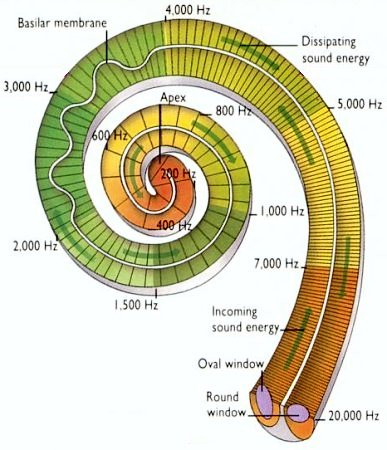
\includegraphics{cochlea}
    \caption{Cochlea divided by frequency regions.}
    \label{fig:cochlea}
\end{figure}

A key factor in the perception of speech and other sounds is \emph{loudness}, a
quality related to the physical property of sound pressure level. Loudness is
quantified by relating the actual sound pressure level of a pure tone (in dB
relative to a standard reference level) to the perceived loudness of the same
tone (in a unit called phons) over the range of human hearing (20 Hz–20 kHz)
\cite{rabiner.schafer.2007}. As shown in \figureref{loudness}, a 100 Hz tone
at 60 dB is equal in loudness to a 1000 Hz tone at 50 dB, both having the
\emph{loudness level} of 50 phons (by convention).


\begin{figure}[ht]
    \centering
    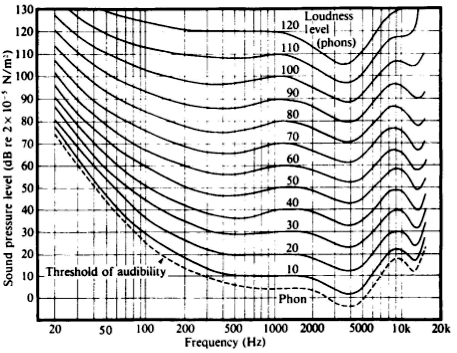
\includegraphics[width=\textwidth]{loudness}
    \caption{Loudness level for human hearing \cite{fletcher.munson.1933}.}
    \label{fig:loudness}
\end{figure}


\subsection{The Mel Scale}

The mel scale is the result of an experiment conducted by Stevens, Volkmann and
Newman \cite{stevens.volkmann.newman.1937} intended to measure the perception
of a pitch and construct a scale based on it. Each observer was asked to listen
to two tones, one in the fixed frequencies 125, 200, 300, 400, 700, 1000, 2000,
5000, 8000 and 12000 Hz, and the other free to have its frequency varied by the
observer for each fixed frequency of the first tone. An interval of 2 seconds
separated both tones. The observers were instructed to say in which frequency the
second tone was ``half the loudness" of the first. A geometric mean was taken from
the observers' answers and a measure of 1000 mels was assigned to the frequency
of 1000 Hz, 500 mels to the frequency sounding half as high (as determined by Fig. 1
in \cite{stevens.volkmann.newman.1937}) and so on.

Decades after the creation of the mel scale, O'Shaughnessy \cite{oshaughnessy.1987}
published an equation to convert frequencies in hertz to frequencies in mels.

\begin{equation}
    f_{mel} = 2595 log_{10}(1 + \frac{f}{700})
    \label{eq:mel_conversion}
\end{equation}
\\
\noindent Being logarithmic, the growth of a mel-frequency curve is slow with a
linear growth of the frequency in hertz. \equationref{mel_conversion} sometimes
is used only for frequencies higher than 1000 Hz while the lower frequencies obey
a linear function. In this work all conversions will use \equationref{mel_conversion},
as shown by \figureref{mel_scale}.

\begin{figure}[ht]
    \centering
    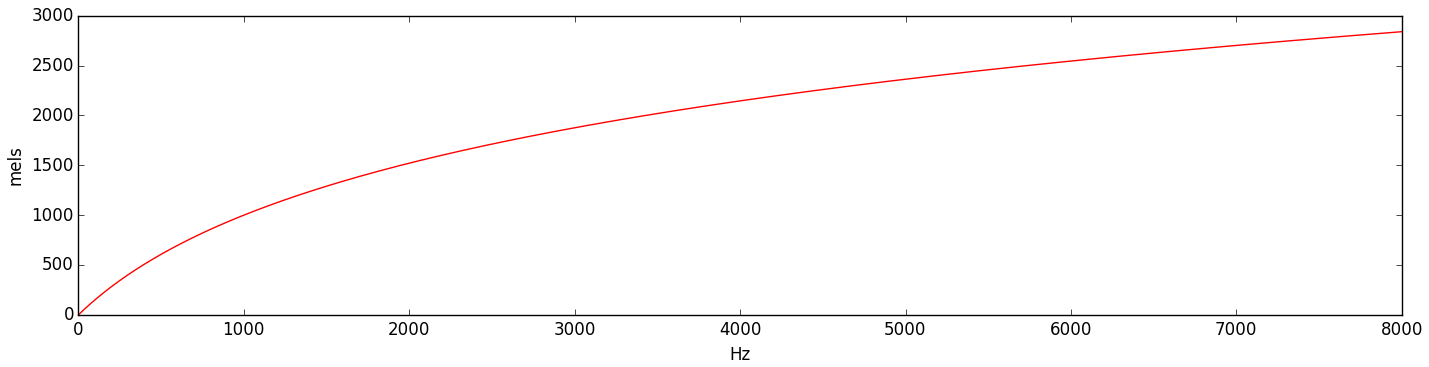
\includegraphics[width=\textwidth]{mel_scale}
    \caption{The logarithm curve of the mel-frequency.}
    \label{fig:mel_scale}
\end{figure}


\subsection{Cepstrum}


\subsection{Extraction Process}


\subsubsection{Pre-emphasis}

\chapter{Gaussian Mixture Model}
\label{ch:gmm}

\chapter{Experiments}
\label{ch:experiments}

The ASR was implemented in its entirety using the programming language Python (version 3.4) and the frameworks NumPy (version 1.8.1) and SciPy (version 0.14.0), meaning the feature extraction, the GMM and UBM models, and the identification and verification classifiers. All codes and data are stored in the public repository \url{https://github.com/embatbr/tg}, as well as this document and secondary resources.

The database used for this work is the \textbf{MIT Mobile Device Speaker Verification Corpus (MIT-MDSCV)}, \refbib{Woo et. al.}{woo.park.hazen.2006}. Two different sets of models were trained. The first was a single speaker GMM for each enrolled speaker, using the utterances relative to the speaker presented in the dataset \textit{enroll\_1}. The trainings took 2-12 seconds each, by the EM algorithm. The second set was of UBMs, also using the utterances from the dataset \textit{enroll\_1}. Two types of UBMs were created: an unisex and a divided by gender, both described in \sectionref{ubm} from chapter \chapterref{gmm}. The unisex UBM took 3-6 minutes of training, while the divided by gender took 7-10 minutes. Both sets of models were created and trained for 32, 64 and 128 distributions, 6, 13 and 19 cepstral coefficients and 0, 1 and 2 orders of delta.

Three experiments were conducted: identification, verification using unisex trained UBMs and verification using gender trained UBMs.

\section{Identification}

The identification is performed by the application of \equationref{decision_speaker_identification_3} to vectors of features $\dvec{X}$ extracted from speech signals in \textit{enroll\_2} and models $\lambda_j$ stored in the directory \textit{bases/gmms}. The set of enrolled speakers is composed of all 26 males and 22 females. Each speaker in \textit{enroll\_2} has 54 recorded utterances, with all tested and the percentage of correct identification calculated. TABELA ERRADA!

\begin{table}[h]
    \centering
    \begin{tabular}{|c|c|c|c|c|}
        \hline
        \textbf{Model Order} & \textbf{\#Coeffs.} \multirow{2}{*} & \multicolumn{3}{c|}{\textbf{\#Deltas}} \\ \cline{3-5}
        & & 0 & 1 & 2 \\
        \hline
        \multirow{4}{*}{$M = 32$} & 6 & 29.55 & 40.28 & 51.74 \\ \cline{2-5}
        & 13 & 57.68 & 69.60 & 74.77 \\ \cline{2-5}
        & 19 & 71.76 & 81.52 & 84.53 \\ \cline{2-5}
        \hline
        \multirow{3}{*}{$M = 64$} & 6 & 29.55 & 40.28 & 51.74 \\ \cline{2-5}
        & 13 & 57.68 & 69.60 & 74.77 \\ \cline{2-5}
        & 19 & 71.76 & 81.52 & 84.53 \\ \cline{2-5}
        \hline
        \multirow{2}{*}{$M = 128$} & 6 & 29.55 & 40.28 & 51.74 \\ \cline{2-5}
        & 13 & 57.68 & 69.60 & 74.77 \\ \cline{2-5}
        & 19 & 71.76 & 81.52 & 84.53 \\ \cline{2-5}
        \hline
    \end{tabular}
    \caption{Average correct identification of speakers.}
    \label{table:avg-correctness}
\end{table}

\noindent The values shown in \tableref{avg-correctness} are the mean of the success rates for every speaker in the given configuration.

\section{Verification}

\subsection{Unisex}

\subsection{Gender}

\chapter{Experiments}

\chapter{Conclusion}
\label{ch:conclusion}

TODO escrever a conclusão após terminar tudo (antes do abstract)


%BACKMATTER

\appendix
\chapter{Codes}

\printbibliography

\end{document}